\documentclass[10pt,twocolumn,letterpaper]{article}

\usepackage{cvpr}
\usepackage{times}
\usepackage{epsfig}
\usepackage{graphicx}
\usepackage{amsmath}
\usepackage{amssymb}
\usepackage{subcaption}

% Include other packages here, before hyperref.

\def\q{\mathbf{q}}
\def\p{\mathbf{p}}

% If you comment hyperref and then uncomment it, you should delete
% egpaper.aux before re-running latex.  (Or just hit 'q' on the first latex
% run, let it finish, and you should be clear).
\usepackage[breaklinks=true,bookmarks=false]{hyperref}

\cvprfinalcopy % *** Uncomment this line for the final submission

\def\cvprPaperID{****} % *** Enter the CVPR Paper ID here
\def\httilde{\mbox{\tt\raisebox{-.5ex}{\symbol{126}}}}

% Pages are numbered in submission mode, and unnumbered in camera-ready
%\ifcvprfinal\pagestyle{empty}\fi
\setcounter{page}{4321}
\begin{document}

%%%%%%%%% TITLE
\title{Grasping Affordance}

\author{Maxwell Gray\\
% For a paper whose authors are all at the same institution,
% omit the following lines up until the closing ``}''.
% Additional authors and addresses can be added with ``\and'',
% just like the second author.
% To save space, use either the email address or home page, not both
\and
Ty Trusty\\
\and
Allen Wang\\
\and
Mike Griffin
}
\maketitle
%\thispagestyle{empty}

%%%%%%%%% ABSTRACT
\begin{abstract}
   In this work, we propose to find natural human grasps of objects using a twofold approach, similar to prior work in the domain of full human body affordance, in the spirit of Shape2Pose (ref). The first step is to learn the parameters of several specialized neural networks whose outputs will correspond to an energy over the space of hand configurations, whose minima are designed to correspond to ``natural" grasps. The second is to find a hand pose that corresponds to a local minimum of the learned energy function. (include results here when we have them)
\end{abstract}

%%%%%%%%% BODY TEXT
\section{Introduction}
Affordance has been studied well in the context of human bodies (reference shape2pose here), and has applications to understanding the semantics and function of novel objects. As far as grasping is concerned, only very limited models have been built for very specific objects (ref the paper about how humans actually grasp things). Both problems are typically formulated as optimization problems that involve geometric information about the object as well as prior knowledge about likely poses. For example, the authors of Shape2Pose (ref) define their energy function as a weighted sum of various metrics, including feature compatibility, a pose prior, and several geometric constraints such as self-intersection and distance from assigned contact points. These approaches do use machine learning to an extent, but notably deep learning has not had nearly the impact in this domain that it has elsewhere (e.g., computer vision) (ref Alexnet or something).

On the other hand, there have been several impressive applications of deep neural networks to computational biology, specifically in learning protein-ligand conformation scoring functions (ref those papers we found). These biological fields share certain aspects with the problem of affordance, in the sense that both problems consist of finding optimal pose parameters for one object in terms of the geometry of another. Therefore, although we do not directly use the approaches found in the biological literature, we take inspiration from this success in formulating our own approach to natural human grasps.

\section{Formulation}
The energy function we propose takes the form of a weighted sum of three terms:
\begin{equation}
E(\q) = w_{\text{pose}}E_{\text{pose}}(\q) + w_{\text{feat}}E_{\text{feat}}(\q)+ w_{\text{dist}}E_{\text{dist}}(\q)
\end{equation}
where $\q$ is the hand configuration, and $E$ is an object-dependent energy function, $E = E[X]$ for an object $X$. In practice the hand configuration is a vector of joint angles as well as a root position in space, and we represent the objects as both point clouds and triangular meshes for separate purposes.

\subsection{Pose Prior ($E_{\text{pose}}$)}
The energy $E_{\text{pose}}$ plays a similar role to the direct pose prior in the original Shape2Pose work, in that it represents a distribution over natural human poses. However, rather than directly fitting a normal distribution to training poses, we train an Energy-Based Generative Adversarial Network (EBGAN) (ref) with an autoencoder as its discriminator and use the discriminator's reconstruction error for this energy term. The authors of the EBGAN paper note that the discriminating autoencoder can be seen as being regularized by contrastive samples from the generator, leading to a better representation of the input distribution. This intuition, as well as the autoencoder's ability to represent complex distributions, motivates this energy term.

\subsection{Feature Compatibility ($E_{\text{feat}}$)}
Again we draw inspiration from the original Shape2Pose, where feature compatibility is defined in terms of a negative log likelihood that a body part contacts the object at a point $p$:
\begin{equation}
	E_{\text{feat, S2P}} = -\sum_{p \in \text{Body}} \log V_p(m(p))
\end{equation}
where $V_p$ is a random forest regression model for the probability that a part $p$ makes contact with the assigned point $m(p)$.

The corresponding energy in our formulation is parameterized by a neural network rather than a random forest. In particular, we use a PointNet++ network (ref) to predict the log probability that each point on the mesh is the nearest point to each joint or end effector on the hand. An important difference between our formulation and that of Shape2Pose is that we do not directly predict contacts in this way; we simply score based on nearest points.

\subsection{Distance ($E_{\text{dist}}$)}
A distance penalty is imposed on the hand for the sum of the distances from each joint and end effector to its nearest point.
\begin{equation}
E_{\text{dist}}(\q) = \sum_{i=1}^k ||\p_i - x_i(\q)||^2_2
\end{equation}
\begin{equation}
\text{where } \p_i = \arg \min_{\p' \in \text{Object}} ||\p' - x_i(\q)||^2_2
\end{equation}
and $x_i(\q)$ is the position of the $i$th joint, and $k$ is the number of such joints.
In this way, despite random initialization, our energy will assign higher scores to configurations near to the object, as we expect a grasp should be.


\section{Learning the Energy}
\subsection{Pose Prior}
To learn a prior over poses, we trained an EBGAN model (ref) on joint angles extracted from the Columbia GraspIt dataset (ref). The goal of the EBGAN is the same as the original GAN formulation, which is to simultaneously train a generator and discriminator. The discriminator must distinguish real samples from a dataset from fake samples from the generator. On the other hand, the generator uses input from random noise to produce fake samples that should be indistinguishable from real data samples. 

However, the main difference of the EBGAN from the original GAN is the treatment of the discriminator as an energy function. The goal of the discriminator then changes to assigning low energies to real samples and assigning high energies to fake samples. The energy model can vary, but in our case (and in the original paper) an autoencoder is trained with the reconstruction loss being treated as the energy. Given a positive margin $m$, a data sample $x$, and a generated sample $G(z)$, the loss function of this system becomes
\begin{equation}
\mathcal{L}_D(x,z) = D(x) + [m - D(G(z))]^+
\end{equation}
\begin{equation}
\mathcal{L}_G(z) = D(G(z)) + f_{PT}
\end{equation}
\begin{equation}
\label{eq:repel}
f_{PT}(S) = \frac{1}{N(N-1)}\sum_i \sum_{i \neq j} \left( \frac{S_i^T S_j}{\|S_i \| \| S_j \|} \right)^2
\end{equation}
where $[\cdot]^+=\max(0, \cdot)$, and $f_{PT}$ [\ref{eq:repel}] represents a repelling regularizer term to prevent mode collapse by orthogonalizing the pairwise sample representation of a mini-batch $S$. The original EBGAN authors note that if the system reaches a Nash equilibrium, then the generator $G$ will produce samples indistinguishable from the distribution of the dataset. The architecture of the model can be seen in Table \ref{table:ebganarch}.
\begin{table*}[h!]
\caption{Model architectures of the EBGAN model. $N$ represents the batch size.}
\label{table:ebganarch}
\captionsetup[subtable]{position = below}
\captionsetup[table]{position=top}
\centering
\begin{subtable}{0.33\linewidth}
\begin{tabular}{ |c|c| }
\hline
layer type & output size \\
\hline
Linear + LeakyReLU & $N \times 16$  \\
\hline
Batch Normalization & $N \times 16 $ \\
\hline 
Linear + LeakyReLU & $N \times 8$ \\
\hline
Batch Normalization & $N \times 8 $ \\
\hline
Tanh & $N \times 8 $ \\
\hline
Linear + LeakyReLU & $N \times 8$  \\
\hline
Batch Normalization & $N \times 8 $ \\
\hline 
Linear + LeakyReLU & $N \times 16$ \\
\hline
Batch Normalization & $N \times 16$ \\
\hline
Tanh & $N \times 16$ \\
\hline
\end{tabular}
\caption{Discriminator's autoencoder architecture}
\end{subtable}
\begin{subtable}{0.33\linewidth}
\begin{tabular}{ |c|c| }
\hline
layer type & output size \\
\hline
Linear + LeakyReLU & $N \times 64$  \\
\hline
Linear + LeakyReLU & $N \times 32$ \\
\hline
Linear + LeakyReLU + 50 \% dropout & $N \times 20$ \\
\hline
Tanh & $N \times 20$\\
\hline
\end{tabular}
\caption{Generator's architecture.}
\end{subtable}
\end{table*}

\subsection{Feature Compatibility}
We also trained the PointNet++ on the Columbia dataset, using example grasps to learn nearest-point probabilities (Mike pls explain how you trained and the class imbalance thing if possible).

\section{Results}
\subsection{Pose Prior}
An example of a generated hand pose and a real hand pose is shown in figure \ref{fig:ebgansamples}. The results for training the EBGAN are shown in Figure \ref{fig:ganresults}. Plotted are the reconstruction distributions, joint angle distributions, and the validation losses for the discriminator and generators. As shown in the figures, the discriminator and generator losses seem to oscillate after around epoch 100, which would imply convergence. Further, the distributions of the reconstruction losses and joint angle distributions seem to match, which appears to be in line with the theoretical results suggested in the original EBGAN paper that the generator would produce results in line with the distribution of the data manifold once a Nash equilibrium is reached. 
\begin{figure}[t]
\caption{EBGAN samples}
\label{fig:ebgansamples}
\centering
\begin{subfigure}[t]{0.23\textwidth}
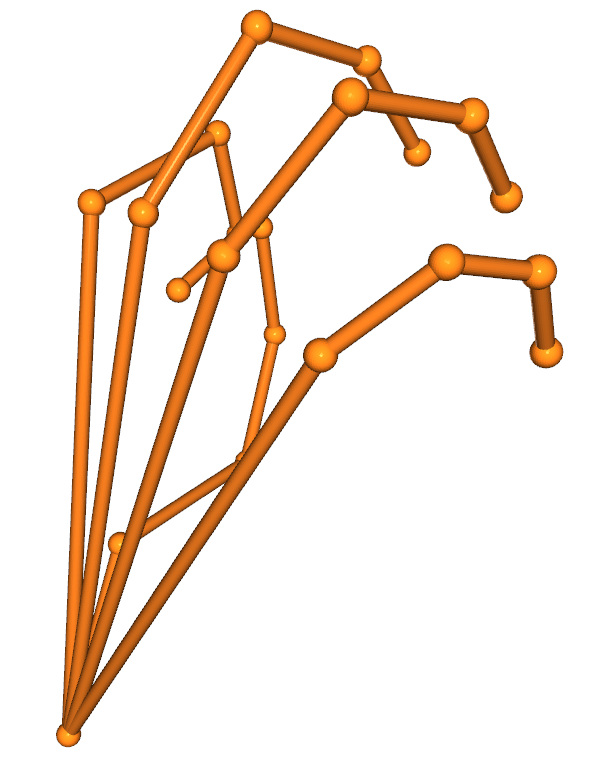
\includegraphics[scale=0.15]{gangenerated.png}
\caption{Generated Hand Pose from EBGAN}
\end{subfigure}
\begin{subfigure}[t]{0.23\textwidth}
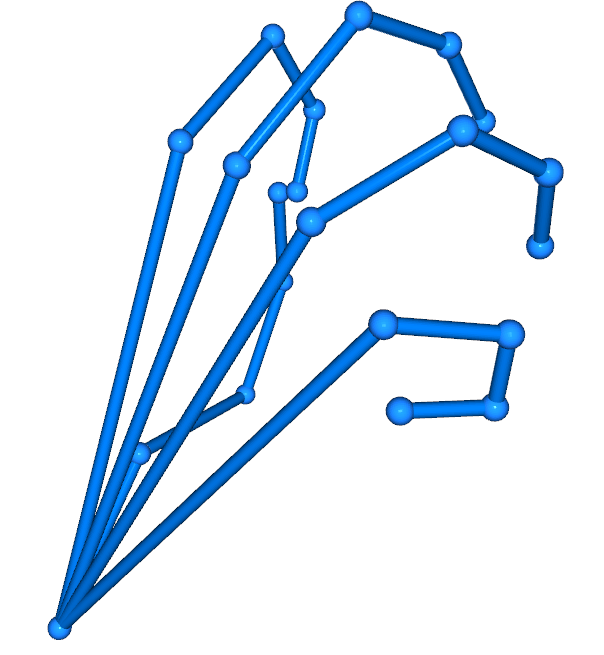
\includegraphics[scale=0.15]{realsample.png}
\caption{Real Hand Pose from Columbia dataset}
\end{subfigure}
\end{figure}

\begin{figure*}[h]
\centering
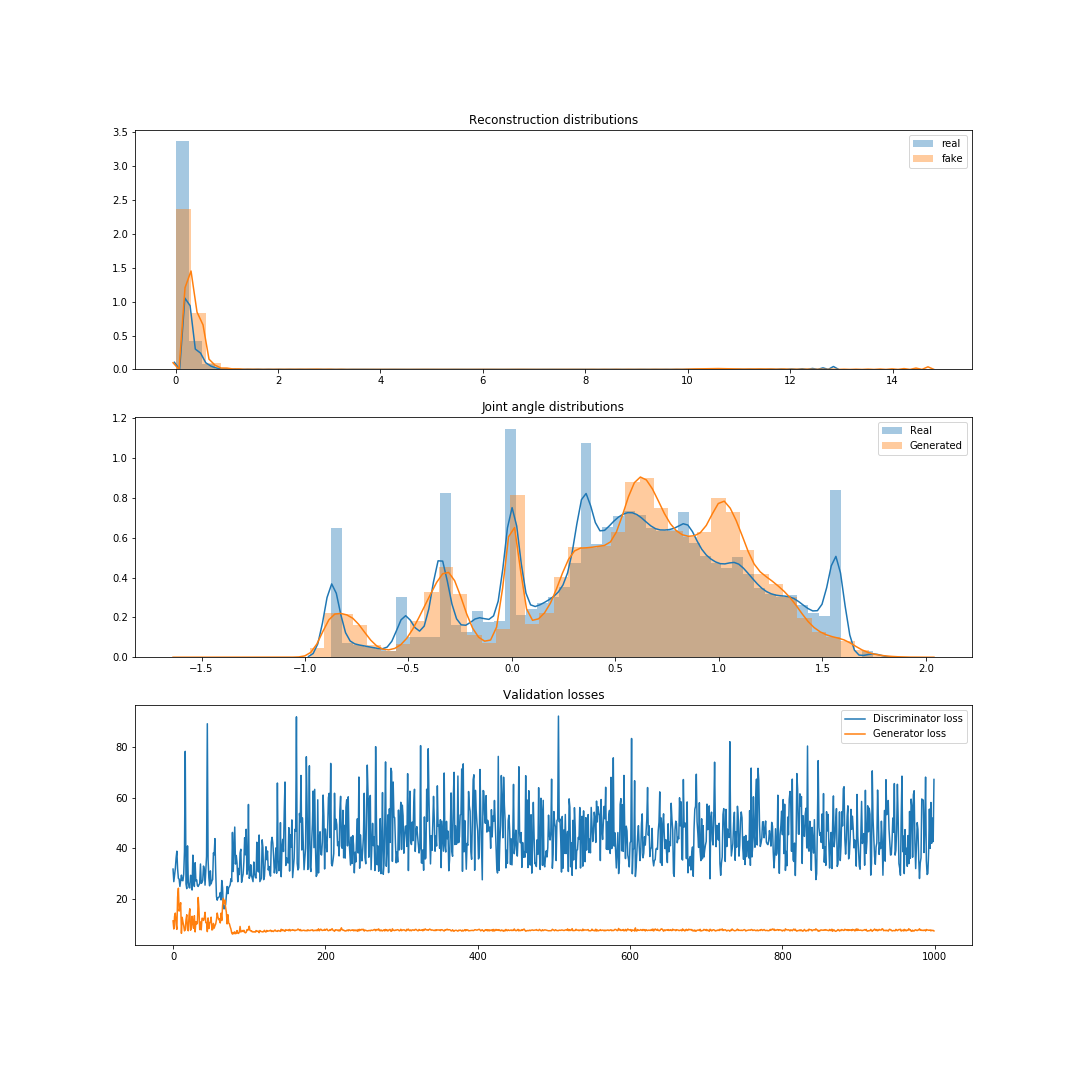
\includegraphics[scale=0.45]{gan_res.png}
\caption{EBGAN training results}
\label{fig:ganresults}
\end{figure*}
\section{Discussion}

%------------------------------------------------------------------------

{\small
\bibliographystyle{ieee}
\bibliography{egbib}
}

\end{document}
